\documentclass[preprint]{emulateapj}
%%GB: General commands to make editing easier and with less typos.

%% -----------------------------------------------
%% Definition of a forloop command
%%
%% This is called via: 
%%   \forloop[step]{counter}{initial_value}{conditional}{code_block} 
%%
\newcommand{\forloop}[5][1]%
{%
\setcounter{#2}{#3}%
\ifthenelse{#4}%
	{%
	#5%
	\addtocounter{#2}{#1}%
	\forloop[#1]{#2}{\value{#2}}{#4}{#5}%
	}%
% Else 
	{%
	}%
}% 

%% -----------------------------------------------
%% Editing
\newcommand{\tbd}[1]{{\par\bf\textsc{TBD: #1\\}}}
\newcommand{\ctbd}[1]{}
\newcommand{\corr}{\textcolor{red}{(corr?) }}
\newcommand{\spl}{\textcolor{red}{(spl?) }}

%% ------------------------------------------------
%% Hun characters
\newcommand{\ii}{\'\i }
\newcommand{\oo}{\H{o}}
\newcommand{\uu}{\H u}

%% --------------------------------------
%% Often used. 
\newcommand{\lc}{light curve}
\newcommand{\lcs}{light curves}
\newcommand{\Lc}{Light curve}
\newcommand{\Lcs}{Light curves}
\newcommand{\avg}[1]{\ensuremath{\langle #1\rangle}}
\newcommand{\med}[1]{\ensuremath{\langle #1\rangle_{med}}}
\newcommand{\dpt}{data-point}
\newcommand{\dpts}{data-points}
\newcommand{\tel}{telescope}
\newcommand{\magn}{magnitude}
\newcommand{\stan}{standard}
\newcommand{\aper}{aperture}
\newcommand{\oot}{out-of-transit}
\newcommand{\OOT}{Out-of-Transit}
\newcommand{\cfa}{Harvard-Smithsonian Center for Astrophysics (CfA)}
\newcommand{\cfadigi}{CfA Speedometers}
\newcommand{\cmd}{color-magnitude diagram}

%% ---------------------------------------------
%% 
\newcommand{\conc}[1]{\noindent\par{\noindent{$\mathbf \Longrightarrow$ \bf #1}}}
\newcommand{\diam}{\ensuremath{\oslash}}
\newcommand{\ccdsize}[1]{\ensuremath{\rm #1\times\rm#1}}
\newcommand{\fovsize}[2]{\ensuremath{\rm #1 #2\times\rm#1 #2}}
\newcommand{\tsize}[1]{\mbox{\rm #1 m}}
\newcommand{\band}[1]{\ensuremath{#1}~band}
\newcommand{\sband}[1]{\ensuremath{#1}}
\newcommand{\ordo}{\ensuremath{\mathcal{O}}}
\newcommand{\chisq}{\ensuremath{\chi^2}}
\newcommand{\RA}[3]{\ensuremath{#1^{\mathrm h}#2^{\mathrm m}#3^{\mathrm s}}}
\newcommand{\DEC}[3]{\ensuremath{#1^{\mathrm d}#2^{\mathrm m}#3^{\mathrm s}}}

%% ---------------------------------------------------------------------
%% Dimensions/quantities
\newcommand{\ghr}{\ensuremath{^h}}
\newcommand{\gmin}{\ensuremath{^m}}
\newcommand{\Ks}{\ensuremath{K_s}}
\newcommand{\masy}{\ensuremath{\rm mas\,yr^{-1}}}
\newcommand{\kms}{\ensuremath{\rm km\,s^{-1}}}
\newcommand{\ms}{\ensuremath{\rm m\,s^{-1}}}
\newcommand{\msd}{\ensuremath{\rm m\,s^{-1}\,d^{-1}}}
\newcommand{\mss}{\ensuremath{\rm m\,s^{-2}}}
\newcommand{\gcmc}{\ensuremath{\rm g\,cm^{-3}}}
\newcommand{\ergscmsq}{\ensuremath{\rm erg\,s^{-1}\,cm^{-2}}}
\newcommand{\C}{\ensuremath{^{\circ}C\;}}
\newcommand{\el}{\ensuremath{e^-}}
\newcommand{\sqarcsec}{\ensuremath{\Box^{\prime\prime}}}
\newcommand{\sqarcdeg}{\ensuremath{\Box^{\circ}}}
\newcommand{\pxs}{\ensuremath{\rm \arcsec pixel^{-1}}}
\newcommand{\aduel}{\ensuremath{\lbrack ADU/\el \rbrack}}
\newcommand{\eladu}{\ensuremath{\lbrack \el/ADU \rbrack}}
\newcommand{\adupixs}{\ensuremath{\rm ADU/(pix\, s)}}
\newcommand{\elpixs}{\ensuremath{\rm \el/(pix\, s)}}
\newcommand{\masyr}{\ensuremath{\rm mas\,yr^{-1}}}
%\newcommand{\arcdeg}{\ensuremath{^{\circ}}}


%% ---------------------------------------------------------------------
%% General
\newcommand{\msini}{\ensuremath{m \sin i}}
\newcommand{\mplsini}{\ensuremath{\mpl\sin i}}
\newcommand{\teff}{\ensuremath{T_{\rm eff}}}
\newcommand{\logg}{\ensuremath{\log{g}}}
\newcommand{\vsini}{\ensuremath{v \sin{i}}}
\newcommand{\feh}{\ensuremath{\rm [Fe/H]}}
\newcommand{\logl}{\ensuremath{\log{L}}}
\newcommand{\vmac}{\ensuremath{v_{\rm mac}}}
\newcommand{\vmic}{\ensuremath{v_{\rm mic}}}
% Activity index R'_HK
\newcommand{\rhk}{\ensuremath{R^{\prime}_{\rm HK}}}
% log of R'_HK
\newcommand{\logrhk}{\ensuremath{\log\rhk}}
% S average value
\newcommand{\Savg}{\ensuremath{\langle S\rangle}}
% Some magnitude differences
\newcommand{\vic}{\ensuremath{V\!-\!I_C}}
\newcommand{\ebv}{\ensuremath{E(B\!-\!V)}}

%% ---------------------------------------------------------------------
%% Solar quantities 
\newcommand{\rsun}{\ensuremath{R_\odot}}
\newcommand{\msun}{\ensuremath{M_\sun}}
\newcommand{\lsun}{\ensuremath{L_\sun}}
\newcommand{\loglsun}{\ensuremath{\log{L_\sun}}}
\newcommand{\teffsun}{\ensuremath{T_{eff,\sun}}}
\newcommand{\rhosun}{\ensuremath{\rho_\sun}}
\newcommand{\loggsun}{\ensuremath{\log{g_{\sun}}}}

%% ---------------------------------------------------------------------
%% Stellar quantities 
\newcommand{\rstar}{\ensuremath{R_\star}}
\newcommand{\mstar}{\ensuremath{M_\star}}
\newcommand{\lstar}{\ensuremath{L_\star}}
\newcommand{\astar}{\ensuremath{a_\star}}
\newcommand{\loglstar}{\ensuremath{\log{L_\star}}}
\newcommand{\teffstar}{\ensuremath{T_{\rm eff\star}}}
\newcommand{\rhostar}{\ensuremath{\rho_\star}}
\newcommand{\loggstar}{\ensuremath{\log{g_{\star}}}}

%% ---------------------------------------------------------------------
%% Earth
\newcommand{\rearth}{\ensuremath{R_\oplus}}
\newcommand{\mearth}{\ensuremath{M_\oplus}}
\newcommand{\learth}{\ensuremath{L_\earth}}
\newcommand{\teffearth}{\ensuremath{T_{\rm eff,\earth}}}
\newcommand{\rhoearth}{\ensuremath{\rho_\earth}}

%% ---------------------------------------------------------------------
%% Planetary
\newcommand{\rpl}{\ensuremath{R_{p}}}
\newcommand{\mpl}{\ensuremath{M_{p}}}
\newcommand{\lpl}{\ensuremath{L_{p}}}
\newcommand{\teffpl}{\ensuremath{T_{\rm eff,{p}}}}
\newcommand{\rhopl}{\ensuremath{\rho_{p}}}
\newcommand{\ipl}{\ensuremath{i_{p}}}
\newcommand{\epl}{\ensuremath{e_{p}}}
\newcommand{\gpl}{\ensuremath{g_{p}}}
\newcommand{\loggpl}{\ensuremath{\log g_{p}}}

\newcommand{\arstar}{\ensuremath{a/\rstar}}
\newcommand{\zrstar}{\ensuremath{\zeta/\rstar}}

%% ---------------------------------------------------------------------
%% Jupiter
\newcommand{\rjup}{\ensuremath{R_{\rm J}}}
\newcommand{\mjup}{\ensuremath{M_{\rm J}}}
\newcommand{\ljup}{\ensuremath{L_{\rm J}}}
\newcommand{\teffjup}{\ensuremath{T_{eff,{\rm J}}}}
\newcommand{\rhojup}{\ensuremath{\rho_{\rm J}}}
\newcommand{\gjup}{\ensuremath{\g_{\rm J}}}

\newcommand{\rjuplong}{\ensuremath{R_{\rm Jup}}}
\newcommand{\mjuplong}{\ensuremath{M_{\rm Jup}}}
\newcommand{\ljuplong}{\ensuremath{L_{\rm Jup}}}
\newcommand{\teffjuplong}{\ensuremath{T_{eff,{\rm Jup}}}}
\newcommand{\rhojuplong}{\ensuremath{\rho_{\rm Jup}}}
\newcommand{\gjuplong}{\ensuremath{\g_{\rm Jup}}}

%% -----------------------------
%% Software
\newcommand{\pack}[1]{\textsc{\lowercase{#1}}}
\newcommand{\prog}[1]{\texttt{\lowercase{#1}}}
\newcommand{\iraf}{\pack{iraf}}
\newcommand{\todcor}{\prog{todcor}}
\newcommand{\xcsao}{\prog{xcsao}}
\newcommand{\daophot}{\pack{daophot}}
\newcommand{\fihat}{\pack{fihat}}
\newcommand{\fistar}{\prog{fistar}}
\newcommand{\fiphot}{\prog{fiphot}}
\newcommand{\grmatch}{\prog{grmatch}}
\newcommand{\grtrans}{\prog{grtrans}}

%% ---------------------------------------
%% References
%\newcommand{\pref}[1]{p.~\pageref{#1}}
%\newcommand{\figr}[1]{Fig.~\ref{fig:#1}}
%\newcommand{\secr}[1]{\mbox{\S\ \ref{sec:#1}}}
%\newcommand{\eqr}[1]{Eq.~\ref{eq:#1}}
%\newcommand{\tabsr}[1]{Tab.~\ref{tab:#1}}
%\newcommand{\tabr}[1]{\mbox{Table~\ref{tab:#1}}}
%\newcommand{\figrp}[1]{Fig.~\ref{fig:#1} on \pref{fig:#1}}
%\newcommand{\secrp}[1]{\S\ref{sec:#1} on \pref{sec:#1}}
%\newcommand{\eqrp}[1]{Eq.~\ref{eq:#1} on \pref{eq:#1}}
%\newcommand{\tabrp}[1]{Tab.~\ref{tab:#1} on \pref{tab:#1}}

\newcommand{\refp}[1]{p.~\pageref{#1}}

\newcommand{\reffig}[1]{Fig.~\ref{fig:#1}}
\newcommand{\refsec}[1]{\mbox{\S\ \ref{sec:#1}}}
\newcommand{\refeq}[1]{Eq.~\ref{eq:#1}}
\newcommand{\reftab}[1]{Tab.~\ref{tab:#1}}

\newcommand{\reffigl}[1]{Figure~\ref{fig:#1}}
\newcommand{\refsecl}[1]{\mbox{Section \ref{sec:#1}}}
\newcommand{\refeql}[1]{Equation~\ref{eq:#1}}
\newcommand{\reftabl}[1]{Table~\ref{tab:#1}}

\newcommand{\reffigp}[1]{\reffig{#1} on \pref{fig:#1}}
\newcommand{\refsecp}[1]{\refsec{#1} on \pref{sec:#1}}
\newcommand{\refeqp}[1]{\refeq{#1} on \pref{eq:#1}}
\newcommand{\reftabp}[1]{\reftab{#1} on \pref{tab:#1}}

\newcommand{\reffigls}[2]{Figures~\ref{fig:#1}--\ref{fig:#2}}
\newcommand{\reftabls}[2]{Tables~\ref{tab:#1}--\ref{tab:#2}}

%% --------------------------------------
%% Instruments
% 
%% FLWO 1.2 m telescope
\newcommand{\flwof}{\mbox{FLWO 1.2\,m}}

%% FLWO 1.5 m telescope
\newcommand{\flwos}{\mbox{FLWO 1.5\,m}}

%% TopHAT 0.25m telescope
\newcommand{\flwot}{\mbox{TopHAT 0.25\,m}}

%% MMT
\newcommand{\mmt}{\mbox{MMT 6.5\,m}}

%% Spitzer
\newcommand{\ssts}{{\em Spitzer}}
\newcommand{\sstL}{{\em Spitzer Space Telescope}}

%% HST
\newcommand{\hst}{{\em HST}}

%% Wise 1m
\newcommand{\wom}{\mbox{Wise 1\,m}}

\newcommand{\piszkessch}{Konkoly 0.6\,m Schmidt}
\newcommand{\piszkesrcc}{Konkoly 1\,m RCC}


%% --------------------------------------
%% Variable types
%% 
\newcommand{\dscu}{\mbox{$\delta$ Scuti}}
\newcommand{\gdor}{\mbox{$\gamma$ Dor}}

\newcommand{\hj}{hot Jupiter}
\newcommand{\vhj}{very hot Jupiter}

% ---------------------------------------------------------------------
%% Astronomical catalogues

%% HD: 
\newcommand{\hd}[1]{\mbox{HD #1}}

%% BD
\newcommand{\BD}[1]{\mbox{BD #1}}

%% HIP
\newcommand{\hip}[1]{\mbox{HIP #1}}

%% GJ
\newcommand{\gj}[1]{\mbox{GJ #1}}

% ---------------------------------------------------------------------
% Shorthand
\newcommand{\tbn}[1]{\tablenotemark{#1}}

\shorttitle{Spin-orbit misalignment for KOI-368}
\shortauthors{shortauthors}


%%% packages
\usepackage{graphicx}
\usepackage{amsmath}
\usepackage{xspace}
\usepackage{subfigure}
%\usepackage{array}
\usepackage{lineno}

\newcommand{\myemail}{email@email.com}

\begin{document}
\linenumbers

\title{Spin-orbit misalignment for the long period planet candidate KOI-368.01}

\author{First Author\altaffilmark{1} and
Second Author\altaffilmark{2}}

\altaffiltext{1}{Affil2; \email{\myemail}}
\altaffiltext{2}{Affil1}

\begin{abstract}
Abstract
\end{abstract}

\keywords{keywords}

\section{Introduction}
\label{sec:introduction}

\citet{Hirano:2012} 
using the rotation period from the \lc\ and 
then combined with the projected rotation period and stellar radius from 
high-res spectroscopy, measured the obliquity of 15 KOI systems. 

\citet{Barnes:2011} use the asymmetry in the Kepler transit \lc\ of 
KOI-13 to measure the spin-orbital alignment angle. 

%\section{Method}
%\label{sec:method}

%The gravity darkening model

\section{KOI-368 stellar parameters}
\label{sec:host-star-parameters}

{\bf KOI-368} is assigned as an Kepler Object of Interesting (KOI) in the 
\citet{Batalha:2013} Kepler catalog from the Quarter 1-6 data. It has a 
Kepler Input Catalog (KIC) entry 6603043. The KIC parameters of the star are 
$T_{\rm eff} = 9034 {\rm K}$, $\rm logg=4.133$, and $\rm FeH = -0.028$, 
indicating it is a hot and fast rotating star.

We took an high resolution (R$\sim$31500) spectrum of this star using 
the ARC Echelle Spectrograph mounted on the Apache Point Observatory  
3.5-meter telescope (APO 3.5m).
[APO observation and spectrum fitting]

The host star rotation period can be identified by searching for spot
modulation in the Kepler Long Cadence PDC \lcs\ \citep{Smith:2012} 
from Q1-Q9. We masked out the primary transits and performed a Lomb-Scargle 
periodogram \citep[][]{Lomb1976,Scargle1982} analysis
on the \lcs. A significant peak at 1.19 days was identified,
and checked by the CLEAN algorithm \citep{Roberts1987}. [This peak 
corresponds with vsini and was adopted as the rotation period of the star].

% \begin{figure}[h!]
%   \centering
%   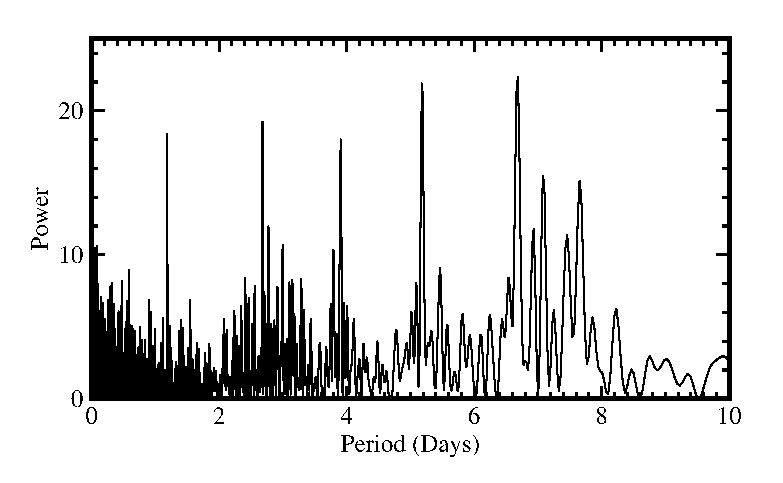
\includegraphics[width=7cm]{LS.eps}
%   \caption{Lomb-Scargle periodogram of the PDC lightcurve, with the
%     transits masked out. The lightcurve is rotationally modulated with
%   a period of 1.19 days.}
%   \label{fig:LS}
% \end{figure}

\section{Orbit obliquity from light curve asymmetry}
\label{sec:transit-light-curve}

\subsection{Light curve model}
\label{sec:lightcurve-model}

We make use of the all the available public Kepler \lcs\ for our analysis 
of the photometry effect predicted by \citet{Barnes:2009}. These include 
Long Cadence (29.4min) data (Q0-Q15) and Short Cadence (58.84s) data (Q8-Q9). 
The long cadence \lcs\ consist of 11 transit altogether (assigned 
transit number from epoch 0-11, the 7th transit is not observed by Kepler 
due to data gap). The short cadence \lcs\ have transit 5 and 6. 

We start with the $\rm SAP\_FLUX$ obtained from the MAST arxive  
\footnote{http://archive.stsci.edu/kepler/data$\_$search/search.php}, the out 
of transit variations are corrected by the following steps from 
\citet{Huang:2013}:

a) removal of bad data points;

b) correction of safe mode and tweaks;

c) a set of cosine functions with minimum period of 1 day. 

d) a 7th order polynomial fit on the out of transit parts. 
\begin{figure}
  \centering
  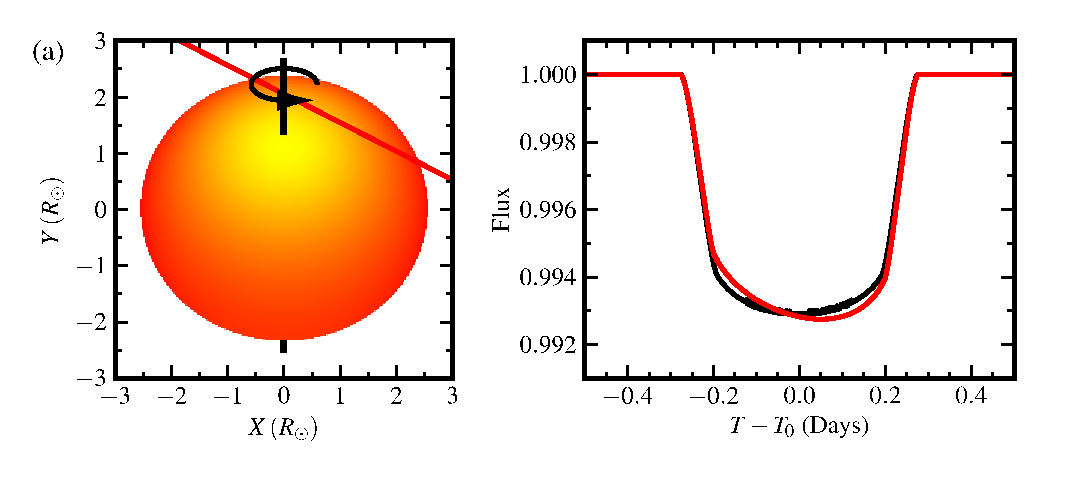
\includegraphics[width=9cm]{obliq_model.eps}
  \caption{f=0.2,$\beta=1.0$, $i_{\rm rot}=0$. Model using koi-368 system
    parameters (inc, rsum, rratio etc). 0, 45, 90 degree obliquity.}
  \label{fig:obliqmodel}
\end{figure}

%\begin{figure}[h!]
%  \centering
%  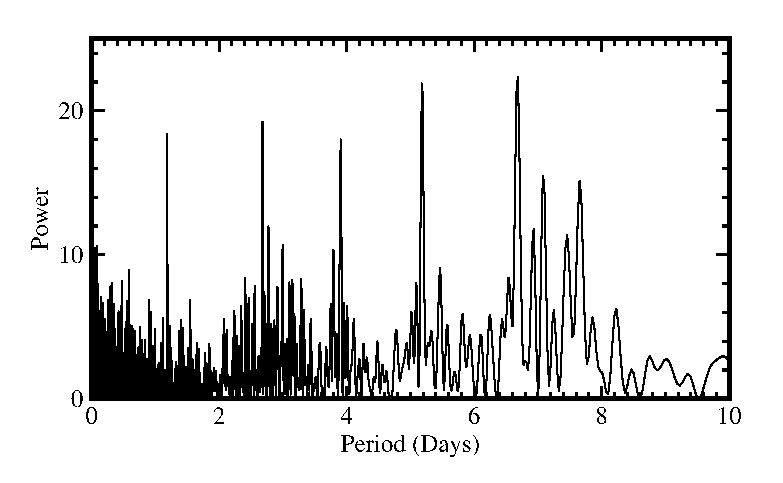
\includegraphics[width=7cm]{LS.eps}
%  \caption{Lomb-Scargle periodogram of the PDC lightcurve, with the
%    transits masked out. The lightcurve is rotationally modulated with
%  a period of 1.19 days.}
%  \label{fig:LS}
%\end{figure}

\subsection{Gravity darkening modeling}
\label{sec:grav-model}
The gravity darkening model is generated following \citet{Barnes:2009}.
The temperature profile on the stellar surface is determined by the local 
effective gravity \citep{Zeipel:1924}. 
\begin{equation}
\frac{T}{T_{\rm pole}} \propto (\frac{g_{\rm eff}}{g_{\rm pole}})^{\beta} 
= F_{f,w} (r,\theta).
\end{equation}
The the effective gravity is defined as 
\begin{equation}
\vec{g}_{\rm eff} = -\Omega_{\rm grav}^2\frac{R_{\rm eq}^3}{R^2}\hat{r} \\ 
+ \Omega_{ror}^2\,R_{\perp}\hat{r_{\perp}}
\end{equation}
We use $\Omega_{\rm ror}$ to measure the stellar rotation rate in radians 
per second and $\Omega_{\rm grav}$ to represent the angular velocity due to 
gravity at the equator, $\Omega_{\rm grav}^2 = GM/R_{\rm eq}^3.$). 
The definition of the other symbols follow \citet{Barnes:2009} Eq.10, in 
which $G$ is the gravitational constant, $M$ is the mass of the star, $R$ 
and $R_{\perp}$ are the distance from the stellar center and stellar 
rotation axis to the point of question, respectively. $\hat{r}$ and 
$\hat{r_{\perp}}$ are unit vectors indicate the directions of $R$ and 
$R_{\perp}$. 
The effective gravity profile $\frac{g_{\rm eff}}{g_{\rm pole}}$ at the stellar 
surface is a function of the oblation of the star $f$, defined as 
$\frac{R_{\rm eq}-R{\rm pole}}{R_{\rm eq}}$, the non-dimension 
measure of the rotation rate ($w=\Omega_{ror}/\Omega_{grav}$, 
and the normalized position parameters $r$ and $\theta$. The 
We use the gravity darkening coefficient computed 
for Kepler band using ATLAS code from \citet{Claret:2011}. By assuming the 
distribution of errors in the stellar parameters to be gaussian, we obtain 
the gravity darkening parameter $\beta$ to be ?.
We demonstrate the flux profile computed for KOI-368 system with $f=0.2$, 
$\beta=1.0$ and assuming the stellar rotation axis is in the plane 
perpendicular to our line of site ($i_{\rm rot}=0$) in Figure 
\ref{fig:obliqmodel}. If the planet cross the hotter pole to colder 
equator during its transits, the transit \lcs\ will show asymmetry depend 
on the misalignment between the planet orbit and stellar rotation axis.


\subsection{System parameter fitting}
\label{sec:model-fitting}

The transit \lcs\ are modeled using the
\citet{Nelson1972} model, implemented in an adaption of the
JKTEBOP code \citep{Proper1981,Southworth2004}. The
relevant free parameters are orbital period $P$, transit centre $T_0$,
normalised radius sum $R_\star+R_p / a$, radius ratio $R_p/R_\star$,
line of sight inclination $i$. Quadratic limb darkening coefficients,
$c_1$ and $c_2$, are fitted for in an initial minimization routine, with 
initial estimates taken from \citet{Sing2010}, then held fixed for 
subsequent analyses. Jump parameters for the stellar oblation correction 
include the planet orbit obliquity $\lambda$, stellar oblation $f$. The 
projection angle between the stellar rotation axis and line of sight 
$i_\text{rot}$ is fixed for an initial analysis, then set free to explore 
the potential degeneracies. The gravity darkening exponent $\beta$ is set 
to be fixed at (? see Section \S \ref{sec:grav-model}), but also allowed 
free in subsequent analysis to explore degeneracies. A flux offset for each 
transit event is calculated and removed at each iteration, and is not 
included in the fit parameters. For Kepler long cadence data, the model is 
modified by a 30 minute boxcar smooth. The best fit parameters and the 
posterior probability distribution is explored via a Markov chain Monte Carlo
(MCMC) analysis, using the \emph{emcee} MCMC ensemble sampler
\citep{ForemanMackey2012}. The likelihood function is given by
$\exp(-\Delta\chi^2/2)$. For each transit, we scale the flux errors such
that the reduced $\chi^2$ is at unity. This allows for errors other
than photon noise to be taken into account.

Figure~\ref{fig:lightcurve} plots the phase folded transit lightcurve of
KOI-368.01 and the best fit spherical and oblate models. The best fit
spherical host star model cannot explain the significant in-transit
asymmetry observed. 

[compare with Kepler original parameters]
The transit parameter from Kepler catalog is 
$P = 110.3216019$ day and $R=19.16$\rearth.

[restate the finding of oblation]
We find the transit \lcs\ are more consistent with a model of ... 

The best fit parameters are presented in Table~\ref{tab:params}.
The posterior probability distributions for relevant parameters
are plotted in Figure~\ref{fig:posterior}. We find a weak inverse dependency
between $\lambda$ and $\beta$, and a positive dependency between
$\lambda$ and $R_p/R_\star$.

%%% Include parameter table
\begin{deluxetable*}{lrrr}
\tablewidth{0pc}
\tabletypesize{\scriptsize}
\tablecaption{KOI-368 System properties
\label{tab:params}}
\tablehead{
\multicolumn{1}{c}{Parameter} & 
\multicolumn{1}{c}{Spherical Model} &
\multicolumn{1}{c}{Limited Oblate Model} &
\multicolumn{1}{c}{Full Oblate Model} \\
}\startdata
\multicolumn{2}{l}{\textbf{Stellar parameters}}\\ 
$T_\text{eff}$ & $9200\pm500$ & - & -\\
$\log g$ & $4.1\pm0.5$ & - & -\\
$\text{[Fe/H]}$ & $0.0\pm0.5$ & - & -\\
$v \sin i_\text{rot}$ & $100 \pm 10$ & - & -\\
\\
\multicolumn{2}{l}{\textbf{Lightcurve fitting parameters \tablenotemark{1}}} \\ 
Period (Days) & $110.3216229_{-7}^{+3}$& $110.321615_{-6}^{+2}$ & $110.321613_{-7}^{+1}$ \\ 
$T_0$ $(\text{BJD}-2454000)$ & $1030.36382_{-3}^{+2}$& $1030.36407_{-9}^{+6}$ & $1030.36440_{-1}^{+3}$ \\ 
$(R_p+R_\star)/a$ & $0.02101_{-3}^{+1}$& $0.02078_{-5}^{+6}$ & $0.02103_{-2}^{+3}$ \\ 
$Rp/R_\star$ & $0.08401_{-5}^{+4}$ & $0.0866_{-2}^{+1}$ & $0.0854_{-1}^{+1}$ \\
$i$ & $89.209_{-1}^{+2}$ & $89.229_{-4}^{+3}$ & $89.209_{-2}^{+2}$ \\
$f$ & - & $0.064_{-6}^{+3}$ & $0.038_{-2}^{+2}$ \\
$\lambda$ & - & $67_{-7}^{+6}$ & $52_{-7}^{+5}$ \\
$\beta$ & - &- & $0.24_{-3}^{+2}$ \\
$i_\text{rot}$ & - & -  & $25_{-10}^{+4}$ \\
\\
\multicolumn{2}{l}{\textbf{Derived parameters}}\\ 

\enddata
\tablenotetext{1}{Uncertainties quoted are for the last significant figure}
\end{deluxetable*}

\begin{figure}[h!]
  \centering
  \includegraphics[width=9cm]{lightcurve.eps}
  \caption{Top: Phase folded transit lightcurve of KOI-368.01. Long
    cadence observations are plotted in black, short cadence in
    yellow. The best fit transit model for a spherical host star is
    plotted in blue, oblate host star in red. These two models are
    indistinguishable at this scale. Middle: Data residual to the
    spherical host star transit model. The long cadence data are
    plotted in full as gray dots. Long cadence data binned to 1 hour
    intervals are plotted in black, binned short cadence residuals in yellow. Bottom:
    Data residual to the oblate host star transit model.}
  \label{fig:lightcurve}
\end{figure}

\begin{figure*}[h!]
  \centering
  \includegraphics[width=12cm]{posterior.eps}
  \caption{Posterior probability distributions showing the correlation
  between the orbit obliquity $\lambda$ and stellar oblation $f$,
  radius ratio $R_p/R_\star$, gravity darkening exponent $\beta$, sky
  projected angle of the stellar rotation axis $i_\text{rot}$. The
  contours mark the 1 and 2$\sigma$ confidence regions. White contours
mark the distribution for the MCMC analysis with $\beta$ and
$i_\text{rot}$ fixed, the red contours show the distribution with
$\beta$ and $i_\text{rot}$ set free.}
  \label{fig:posterior}
\end{figure*}

\subsection{Asymmetry from eccentricity}
\label{sec:asymm-from-eccentr}

A highly eccentric orbit can also cause asymmetric distortions to the
transit lightcurve. An eccentric orbit distorts the lightcurve by
changing the planet's velocity through the transit. We explore the
possibility that the lightcurve distortions observed for KOI-368.01
are due to an eccentric instead of an oblique orbit.

Following \citet{Barnes2007}, we can constrain the change in velocity
$(\Delta v = v_\text{out} - v_\text{in})$ by measuring the difference
in the duration of ingress and egress $(\Delta t)$,
\begin{align}
  \Delta t &= \frac{R_p}{v_\text{out} \cos\left(\sin^{-1} b \right)} -
  \frac{R_p}{v_\text{in} \cos\left(\sin^{-1} b \right)} \\
  \Delta v &\approx v^2 \frac{\Delta t \cos \left( \sin^{-1} b \right)}{R_p}
\end{align}
where $b = a \cos i/R_\star = 0.7$ is the transit impact parameter, and $v =
\sqrt{G M_\star / a} = 43.3\,\text{kms}^{-1}$. Using
the short cadence data, we measure ingress and egress durations to be
equal to within errors of 0.7 minutes, constraining the maximum
possible change in velocity to be $\Delta v <
0.5\,\text{kms}^{-1}$. Figure~\ref{fig:eccmode} plots the difference 
between such an eccentric orbit lightcurve and its best fit circular orbit
lightcurve. The maximum in-transit distortions are $10
\times$ smaller than that for the oblique orbit model. The maximum
distortions during ingress and egress are $5\times$ smaller than that
for the oblique orbit model, and are not consistent in shape to that
observed for KOI-368.01. The lightcurve distortions for KOI-368.01
therefore cannot be explained by an eccentric orbit.

\begin{figure}[h!]
  \centering
  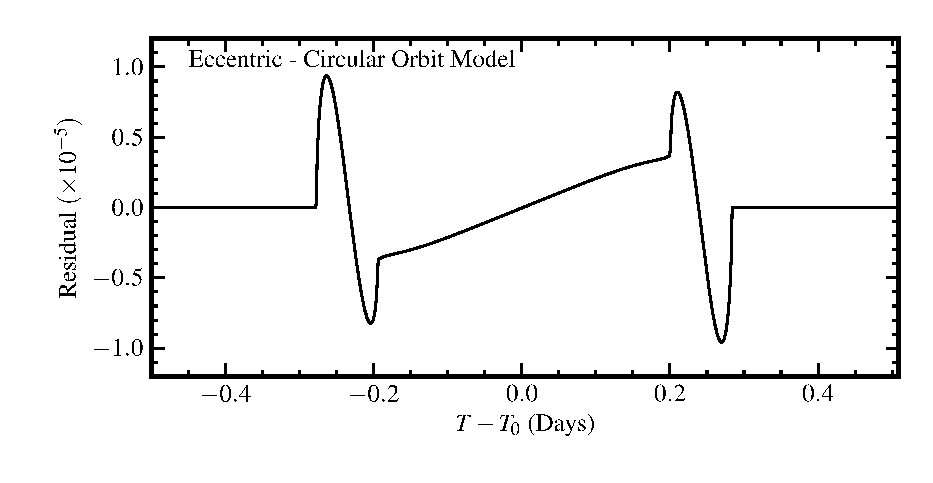
\includegraphics[width=7cm]{ecc_model.eps}
  \caption{The maximum lightcurve distortions due to a
    eccentric orbit for KOI-368.01 are plotted as residuals to its
    best fit circular orbit model. The maximum velocity change is
    determined by measuring the difference in the ingress and egress
    duration. Eccentricity cannot explain the observe lightcurve
    asymmetry (Figure~\ref{fig:lightcurve}, middle panel).}
  \label{fig:ecc_model}
\end{figure}


% \citet{Barnes2007} calculated such an effect for the
% favourablely eccentric hot-Jupiter HD 147506b to be $\sim10^{-6}$ on
% the lightcurve, an order of magnitude
% smaller than the distortions observed for KOI-368.01. We present the
% following arguments that the observed lightcurve distortions for
% KOI-368.01 are not due to an eccentric orbit. 1) KOI-368.01 has an orbital period 20 times longer than that of HD
% 147506b, and will need an orbital eccentricity of $>0.96$ to
% experience the same maximum change in velocity over a transit as that
% HD 147506b. 2) This maximum change occurs directly before or after
% periastron. Such an orbit will cause a transit wiht duration shorter
% than that of a circular orbit. This is contradicted by the measured
% transit duration of KOI-368.01. 3) An eccentric orbit results in
% asymmetric timescales for ingress and egress, which is not observed.


\section{Nature of the companion}
\label{sec:nature-companion}

To establish the planetary nature of KOI-368.01, we investigate in the 
false positive scenarios of this system. We use the image from APO 3.5m 
Echelle Slitviewer camera to rule out close by bright companions. The 
camera has a field of view of 63.6$\arcsec$ and the pixel scale is 0.133\pxs. 
We can rule out companion brighter than 20 mag within 20\sqarcsec\ 
area of KOI-368 (See Figure \ref{fig:APO}). No candidate is found to be 
a possible source of background blend. 

We are able to use the upper limit of centroid displacement to rule out the 
possibility that the transit signal is mimicked by background binaries. We 
use the flux weighted first momentum centroids produced by Kepler 
pipeline. The long time range trend in centroids due to the motion of 
the space craft is corrected by a 7-th order polynomial on each quarter 
of the Long Cadence data. For each Long Cadence transit [do we want to put 
the SC points on as well?], we compare the centroids of star during the 
transit with the centroids before and after the transit (within a window 
of width the same as the transit duration). The displacements between the 
mean centroids of the in-transit part and the out-of-transit part are shown 
in Figure \ref{fig:centroid}. The error-bars are computed with the error 
propagation rule by assuming the centroids in each window follows a 
Gaussian distribution. The analysis shows that the signal could not be 
from a source farther than 1$\arcsec$ away from the star KOI-368.  

A stellar mass M-dwarf companion will cause a secondary eclipse in the
lightcurve. We mask out the primary transit and remove large scale
variations the Kepler long cadence lightcurve using a cosine filter
with minimum width of 1 day. We perform a grid
search for a secondary eclipse, in the phase space between 0.05 and
0.95, using the \citet{Mandel2002} eclipse model. We can rule out the
presence of any secondary eclipse event with depth
$>10^{-5}$. Assuming the system is not a blend, we can constrain the
temperature of the orbiting companion to be $< 2500\,\text{K}$, and
must be of sub-stellar nature.

\subsection{System eccentricity}
\label{sec:system-eccentricity}

The Transit Timing Variation (TTV) analysis for KOI-368.01 with the 
11 transits from Long Cadence data prefer a solution without any high 
amplitude TTV signal (See Figure \ref{fig:TTV}).

The system eccentricity can be constrained by comparing the measured
transit duration $(t_\text{obs}=13.2\,\text{hours})$ against that expected for a circular
orbit \citep[e.g.][]{Barnes2007,Burke2008,Kane2012}. Adopting host star
parameters of $M_\star = 2.2\,M_\odot$ and $R_\star = 2.1\,R_\odot$
[cite/ref], the expected circular orbit transit duration is
$t_\text{circ} =9.8\,\text{hours}$. Following \citet{Burke2008}, we
solve for $e$ in
\begin{equation}
  \label{eq:ecc}
  \frac{t_\text{obs}}{t_\text{circ}} = \frac{\sqrt{1-e^2}}{1+e \cos(\omega-\pi/2)}\,,
\end{equation}
and find $0.3 < e < 1$, depending on the argument of periastron $\omega$. This range is highly
dependent on the assumed host star parameters, which are not well
measured. For a host star with 30\% smaller radius, we find the
eccentricity is constrained to be $>0.9$ for all $\omega$. In the case
of a host star 30\% larger than quoted, we can place no constraints on
eccentricity. 

\begin{figure}
\subfigure[]
{
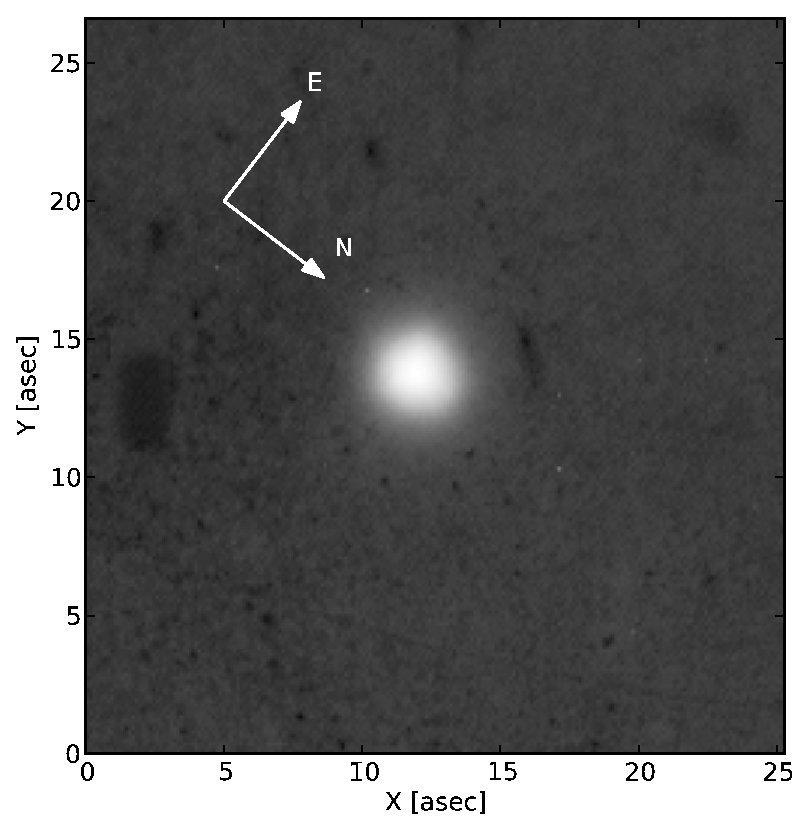
\includegraphics[width=0.45\linewidth]{APOimage.eps}
\label{fig:APO}
}
\subfigure[]{
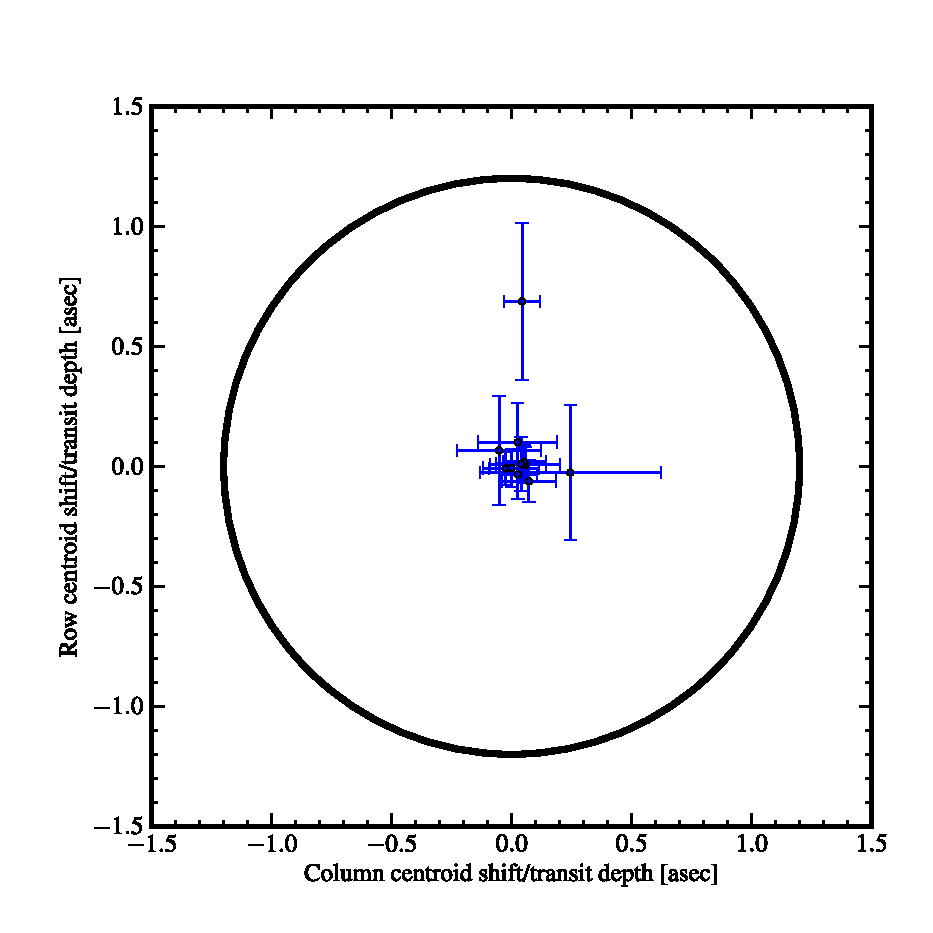
\includegraphics[width=0.45\linewidth]{centroid.eps}
\label{fig:centroid}
}
\end{figure}
\section{Discussion}
\label{sec:discussion}

\begin{figure}
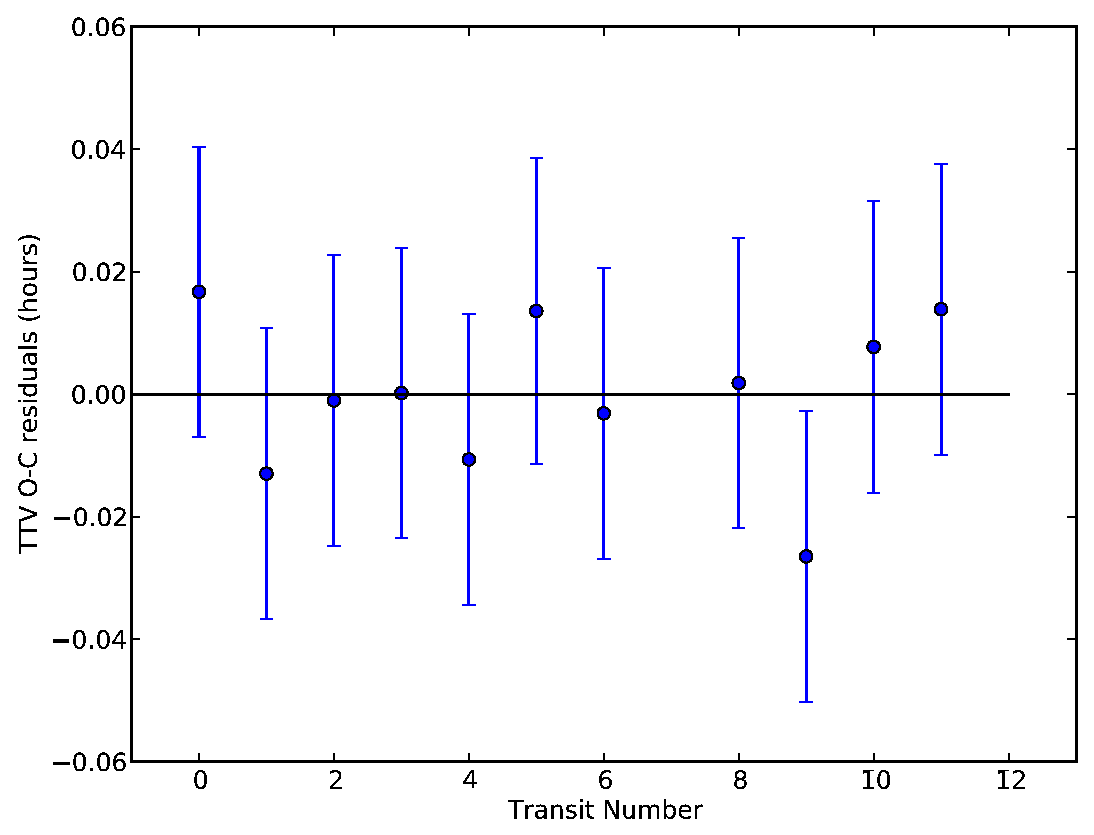
\includegraphics[width=0.9\linewidth]{TTV.eps}
\caption{caption}
\label{fig:TTV}
\end{figure}


\begin{figure}[h]
  \centering
  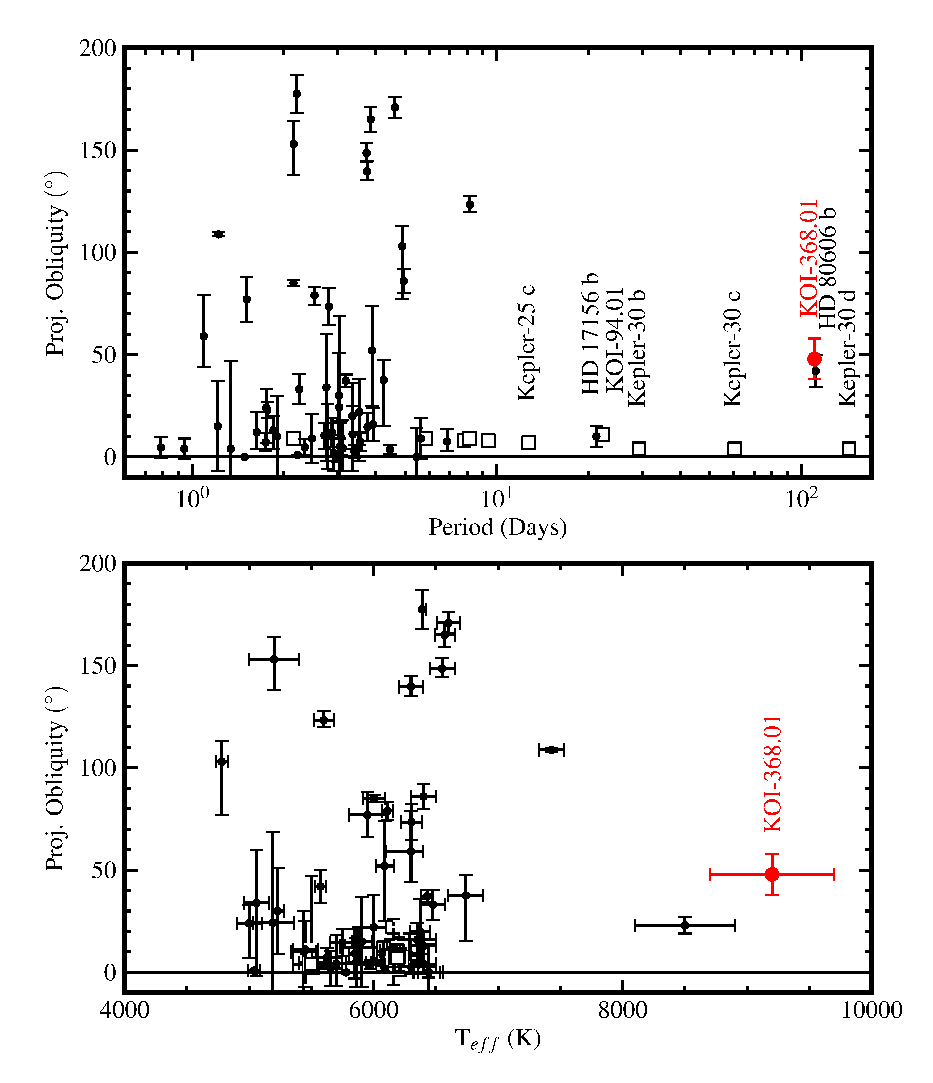
\includegraphics[width=9cm]{period_obliq.eps}
  \caption{caption}
  \label{fig:periodobliq}
\end{figure}

\bibliographystyle{apj}
\bibliography{mybibfile}

\end{document}
